% vim: ts=2:sw=2:tw=80:et
\thispagestyle{fancy}
\pagestyle{fancy}

When the entire waveform has been defined (and hence shown in the plot
viewport), one is ready to begin excuting the waveform.  In the simplest form,
waveform execution is started by selecting the \textit{Play} button in the
toolbar of the main window while the neighboring drop-down box has
\textit{Default} selected (see Fig.~\ref{fig:iterating:select-iter}).  After
presssing \textit{Play}, the \textit{Play} button should change to a
\textit{Stop} button.  Without any other changes, the entire waveform should be
executed with one iteration following immediately after another.  This should
continue until the user selects the \textit{Stop} button.

\begin{figure}[ht!]
  \centerline{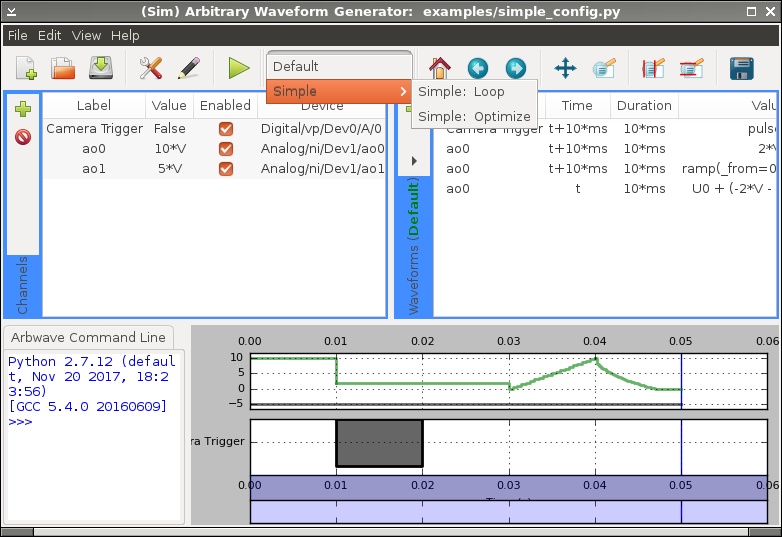
\includegraphics[width=.8\textwidth]{figures/select-iter}}
  \caption[Selecting experimental control loop]{
    Selecting experimental control loop from a list of \textit{runnables}.
  }
  \label{fig:iterating:select-iter}
\end{figure}


More advanced waveform execution modes are also available.  These are modes such
as (nested) for-loops and optimization.  Furthermore, it is possible to define
arbitrary customized code to prepare and respond to each and every iteration of
the experimental waveform--this is particularly necessary when attempting to
optimize a waveform for a particular parameter.  The rest of this chapter will
discuss these more advanced execution modes, while
Sec.~\ref{sec:scripting:runnable} of Chap.~\ref{chap:scripting} will discuss
customized experimental preparation and response code to be executed at each
waveform iteration.

\section{Loops}
As shown in Fig.~\ref{fig:iterating:select-iter}, the drop-down menu, just to
the right of the \textit{Play} button presents a list of the experimental
control loops that define how a single experiment is executed.  Each of these
items is called a \textit{Runnable}.  The \textit{Default} runnable provides for
the output waveforms to be run in continuous iteration mode.  Initially, one
other runnable is defined: the \textit{Simple} runnable.  The implementation of
the \textit{Simple} runnable is shown and discussed in
Sec.~\ref{sec:scripting:simple}.  The \textit{Simple} runnable executes the
waveform one time then quits.

In order to execute this \textit{Simple} runnable in a loop or even nested set
of loops, one selects the \texttt{Simple: Loop} sub-menu item.  Upon
subsequently pressing \textit{Play}, the \textbf{Loop Parameters} dialog is
presented that is depicted in Fig.~\ref{fig:iterating:nested-loops}.  Using this
dialog, it is possible to define simple loops, multiply nested loops, or
sequences of loops.

\begin{figure}[ht!]
  \centerline{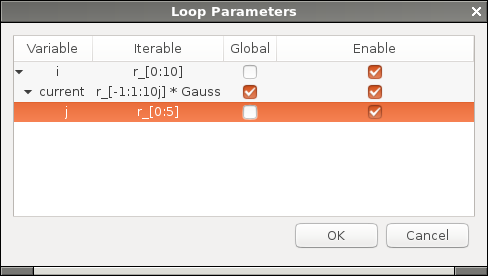
\includegraphics[width=.45\textwidth]{figures/nested-loops}}
  \caption{
    Nested loops for waveform execution.
  }
  \label{fig:iterating:nested-loops}
\end{figure}

\subsection{Variables}

You will find in multiple places that the \textit{Insert} key does special
things like inserting another loop variable.  You can sibling loops, or nested
loops.  You can reorder these by dragging the loop variables.  You can also nest
loops by dragging/dropping loop variables on top of each other.  Furthermore,
while dragging, if you press the \textit{Control} key, the item being dragged
will be copied instead of moved.  This is also a common interface for editing
waveform elements.


\subsubsection{Using Global Variables}
You can use any of the variables defined like in Sec.~\ref{script:variables}
in appropriate waveform elements or even any other place you wish.  In fact,
you can also use these expressions as loop variables if you select "Global" in
the loop editor.  As some examples:

\begin{table}[ht!]
  \center
  \begin{tabular}{p{5cm} m{6cm}c}
  Variable                  &                iterable            &   Global\\
  \hline \hline
  \verb|Bfield[0]|          &       \verb|r_[0:5:3j] * Gauss|      &    X \\
  \verb|Bfield[1]|          &       \verb|r_[5:15:5j] * Gauss|     &    X \\
  \verb|Bfield[2]|          &       \verb|r_[110:130:10j] * Gauss| &    X \\
  \verb|CoilCurrent|        &       \verb|r_[4:5:20j] * A|         &    X \\
  \verb|Frequency['mot']|   &       \verb|r_[-5:-20:5j] * MHz|   &      X \\
  \verb|Frequency['pgc']|   &       \verb|r_[-20:-80:10j] * MHz| &      X \\
  \verb|Frequency['image']| &       \verb|r_[-5:5:10j] * MHz|    &      X \\
  \end{tabular}

  \caption{
    Example of some valid loop variables.
  }
\end{table}


\section{Optimization}
Using the Python SciPy package, Arbwave also provides the means to optimize
experimental parameters.  For the example shown in
Fig.~\ref{fig:iterating:select-iter}, one selects the \texttt{Simple: Loop} sub-menu
item in the \textit{Runnables} drop-down menu.  After subsequently pressing
\textit{Play}, the \textbf{Optimization Parameters} dialog is presented that is
depicted in Fig.~\ref{fig:iterating:optim}.
%
\begin{figure}[ht!]
  \centerline{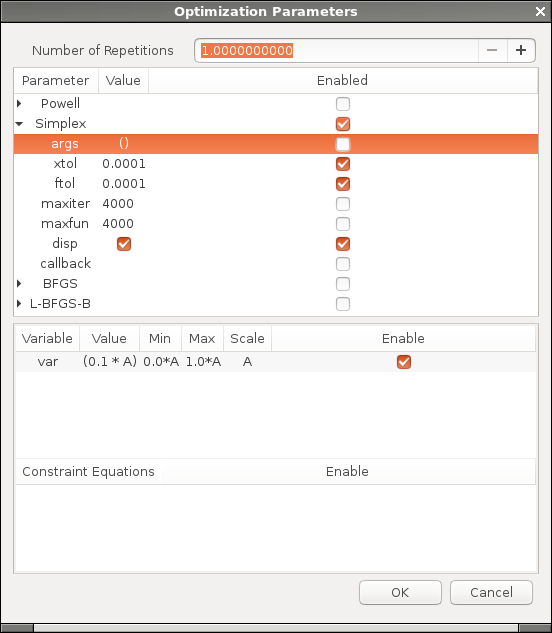
\includegraphics[width=.45\textwidth]{figures/optim}}
  \caption{
    Nested loops for waveform execution.
  }
  \label{fig:iterating:optim}
\end{figure}
%
In this dialog, there are three sections to configure the optimization routines:
\begin{enumerate}
  \item \textit{Algorithms}\\
    Although not all optimization algorithms from the \texttt{scipy.optimize}
    subpackage of the Python SciPy suite, several local and global optimization
    algorithms are enabled for use with Arbwave.  When initially loaded, the
    \textbf{Optimization Parameters} dialog shows all the optimization
    algorithms that can be used by Arbwave.  As shown in
    Fig.~\ref{fig:iterating:optim}, each of the algorithms also includes a
    drop-down list of parameters.  These lists of algorithm parameters allow the
    user to customize the algorithm behavior.  The original documentation from
    Python SciPy should be consulted for modifying these parameters.

    It is possible to enable multiple algorithms that would be executed
    sequentially after another.  Using a drag-drop operation, it is possible to
    re-order these algorithms.  For example, using this re-order feature, one
    can apply a global optimizer followed by a local optimizer.
    It is also possible to copy algorithms in the list, such that multiple
    instances of a certain algorithm can be executed.  As in other parts of the
    Arbwave interface, copying is performed by pressing the \textbf{Control} key
    when dropping an item that is being dragged.

  \item \textit{Variables}\\
    In general, any optimization routine attempts to find the best suited
    parameters for a given merit function.  The list in the \textit{Variables}
    section is the list of values that will be modified by the optimization
    algorithms.  The merit function that defines the performance metric to which
    the variables apply is defined by the \texttt{def run(self):} function of
    a \textit{Runnable} object.  Sec.~\ref{sec:scripting:runnable} discusses how
    to define the value of the merit function that is returned to the
    optimization algorithms.

    As also shown in Fig.~\ref{fig:iterating:optim}, each variable is specified
    by a Python string that can be the left-hand side of an assignment
    operation.  It is thus possible to optimize simple Python variables or even
    more complex expressions, such as a component of an array or member of an
    object.
    
    The \textit{Value} column of a variable represents the initial guess for
    that particular variable and must be specified with units appropriate for
    the variable.  Each variable must also have a valid range specified in the
    \textit{Min} and \textit{Max} columns--also expressed in the same units as
    the variable.  The \textit{Scale} column is a value that is used to each
    variable to a common, unit-less scale.  For example, if two variables,
    \textbf{\textit{a}} and \textbf{\textit{b}} are used, but
    \textbf{\textit{a}} varies from $0$---$100$*A and 
    \textbf{\textit{b}} varies from $-1$---$1$*V, the \textit{Scale} values should
    be expressed as \texttt{100*A} and \texttt{2*V} respectively.

    Note that the \textbf{Insert} key is used to add additional variables.

  \item \textit{Constraint Equations}\\
    It is often also important to apply constraints that are more complicated
    than the range of a single variable.  For instance, consider two variables
    \textbf{\textit{a}} and \textbf{\textit{b}}, where it is desired to keep the
    sum of these variables less than a certain value.  To do this, one would
    (using the \textbf{Insert} key) add a constraint equation such as
    \begin{lstlisting}
    a + b < 3.
    \end{lstlisting}
    Note that the dimensional analysis of the equation must be correct for the
    equation to be evaluated successfully.
\end{enumerate}
